\documentclass[8pt,twocolumn]{article}

\usepackage{../common/cvpr}
\usepackage{times}
\usepackage{epsfig}
\usepackage{graphicx}
\usepackage{amsmath}
\usepackage{amssymb}
\usepackage[normalem]{ulem}
\useunder{\uline}{\ul}{}

% Include other packages here, before hyperref.

% If you comment hyperref and then uncomment it, you should delete
% egpaper.aux before re-running latex.  (Or just hit 'q' on the first latex
% run, let it finish, and you should be clear).
\usepackage[pagebackref=true,breaklinks=true,letterpaper=true,colorlinks,bookmarks=false]{hyperref}

\cvprfinalcopy % *** Uncomment this line for the final submission

% Pages are numbered in submission mode, and unnumbered in camera-ready
\ifcvprfinal\pagestyle{empty}\fi
\begin{document}

%%%%%%%%% TITLE
\title{Progress Report: Mastering Terra Mystica}

%\author{
%Luis Perez\\
%Stanford University\\
%450 Serra Mall\\
%{\tt\small luisperez@cs.stanford.edu}
%}

%\maketitle
\thispagestyle{empty}

%%%%%%%%% ABSTRACT
\begin{abstract}
\label{abstract}
In this progress report, we describe in detail the algorithms and models which we will be using to tackle our proposed problem. For reference, please refer to our previously submitted proposal, which defines and covers the scope of what we wish to achieve.

This paper focuses almost exclusively on describing in detail the methods we've implemented for attempting to achieve our results, as well as very preliminary experimental results we've achieved.

Furthermore, the paper proposes further modification which need to be made, as well as next steps and experiments to be run.
\end{abstract}

%%%%%%%%% BODY TEXT
\section{Background and Overview}
\label{section:background_and_overview}
We provide a brief discussion of our task in this section. For more detail, refer to our previously submitted proposal.

Our task involves developing the infrastructure, framework, and models required to achieve super-human level game-play in the game of Terra Mystica (TM) \cite{TMBoardGeek}, without any of its expansions \footnote{There are multiple expansions, most which consists of adding different Factions to the game or extending the TM Game Map. We hope to have the time to explore handling these expansions, but do not make this part of our goal}. TM is a fully-deterministic, turn-based, strategy board game (though an online implementation exists). The only randomness arises from pregame set-up, such as players selecting different Factions \footnote{A Faction essentially restricts each Player to particular areas of the map, as well as to special actions and cost functions for building}, different set of end-round bonus tiles being selected, as well as other minutia which we discussed in our proposal.

TM is typically played between 2-5 players, though we focused exclusively on the 2-player version of the game.


\section{Deep Q-Learning Methods for Terra Mystica}
\label{section:deep_qlearning_methods_for_tm}
Existing open-source AIs for TM are based on  combination of sophisticated search techniques (such as depth-limited, alpha-beta search, domain-specific adaptations, and handcrafted evaluation functions refined by expert human players). Most of these AIs fail to play at a competitive level against human players. The space of open-source AIs is relatively small, mainly due to the newness of TM.

\subsection{Alpha Zero for TM}
\label{subsection:alpha_zero_for_tm}
In this section, we describe the main methods we use for training our agent. In particular, we place heavy emphasis on the methods described by AlphaGo\cite{AlphaGo}, AlphaGoZero, \cite{AlphaGoZero}, and AlphaZero \cite{AlphaZero} with pertinent modifications made for our specific problem domain.

Our main method will be a modification of the Alpha Zero \cite{AlphaZero} algorithm which was described in detail. We chose this algorithm over the methods described for Alpha Go \cite{AlphaGo} for two main reasons:
\begin{enumerate}
    \item The Alpha Zero algorithm is a zero-knowledge reinforcement learning algorithm. This is well-suited for our purposes, given that we can perfectly simulate game-play. 
    \item The Alpha Zero algorithm is a simplification over the dual-network architecture used for AlphaGo.
\end{enumerate}

As such, our goal is to demonstrate and develop a slightly modified general-purpose reinforcement learning algorithm which can achieve super-human performance tabula-rasa on TM.

\subsubsection{TM Specific Challenges}
\label{subsubsection:tm_specific_challenges}
We first introduce some of the TM-specific challenges our algorithm must overcome.

\begin{enumerate}
    \item Unlike the game of Go, the rules of TM are \textbf{not} translationally invariant. The rules of TM are position-dependent -- the most obvious way of seeing this is that each terrain-tile and patterns of terrains are different, making certain actions impossible from certain positions (or extremely costly). This is not particularly well-suited for the weight-sharing structure of Convolutional Neural Networks.
    \item Unlike the game of Go, the rules for TM are asymmetric. We can, again, trivially see this by noting that the board game board itself \ref{fig:TM_Board} has little symmetry.
    \item The game-board is not easily quantizeable to exploit positional advantages. Unlike games where the AlphaZero algorithm has been previously applied (such as Go/Shogi/Chess), the TM map is not rectangular. In fact, each ``position'' has \textbf{6} neighbors, which is not easily representable in matrix form for CNNs.
    \item The action space is significantly more complex and hierarchical, with multiple possible ``mini''-games being played. Unlike other games where similar approaches have been applied, this action-space is extremely complex. To see this, we detail the action-spaces for other games below.
    \begin{enumerate}
        \item The initial DQN approach for Atari games had an output action space of dimension 18 (though some games had only 4 possible actions, the maximum number of actions was 18 and this was represented simply as a 18-dimensional vector representing a softmax
        probability distribution).
        \item For Go, the output actions space was similary a $19\times19 + 1$ probability distribution over the locations on which to place a stone. 
        \item Even for Chess and Shogi, the action space similarly consisted of all legal destinations of all player's pieces on the board. While this is very expansive and more similar to what we expect for TM, TM nonetheless has additional complexity in that some actions are inherently hierarchical. You must first decide if you want to build, then decided \textbf{where} to build, and finally decide \textbf{what} to build. This involves defining an output actions-space which is significantly more complex than anything we've seen in the literature. For comparison, in \cite{AlphaZero} the output space consists of a stack of planes of $8\times 8 \times 73$. Each of the 64 positions identifies a piece to be moved, with the 73 associated layers identifying exactly \textit{how} the piece will be moved. As can be seen, this is essentially a two-level decision tree (select piece followed by selecting how to move the piece). In TM, the action-space is far more varied.
    \end{enumerate}
    \item The next challenge is that TM is not a binary win-lose situation, as is the case in Go. Instead, we must seek to maximize our score \textit{relative} to other players. Additionally, in TM, there is always the possibility of a tie. 
    \item Another challenge present in TM not present in other stated games is the fact that there exist a limited number of resources in the game. Each player has a limited number of workers/priests/coin with which a sequence of actions must be selected.
    \item Furthermore, TM is now a multi-player game (not two-player). For our purposes, however, we leave exploring this problem to later research. We focus exclusively on a game between two fixed factions (Engineers and Halflings).
\end{enumerate}

\subsection{Input Representation}
\label{subsection:input_representation}
Unless otherwise specified, we leave the training and search algorithm large unmodified from those presented in \cite{AlphaZero} and \cite{AlphaGoZero}. We will described the algorithm, nonetheless, in detail in subsequent sections. For now, we focus on presented the input representation of our game state.

\subsubsection{The Game Board}
\label{subsubsection:the_game_board}

We begin by noting that the TM GameBoard \ref{fig:TM_Board} is naturally represented as $13 \times 9$ hexagonal grid. As mentioned in the challenges section, this presents a unique problem since for each intuitive ``tile``, we have $6$ rather than the the $4$ (as in Go, Chess, and Shogi). Furthermore, unlike chess where a natural dilation of the convolution will cover additional tangent spots equally (expanding to $8$), the hexagonal nature makes TM particularly interesting.

However, a particular peculiarity of TM is that we can think of each ``row'' of tiles as being shifted by ``half'' a tile, thereby becoming ``neighbors''. With this approach, we chose to instead represent the TM board as a $9 \times 26$ grid, where each tile is horizontally doubled. Our terrain representation of the map then begins as a $9 \times 26 \times 8$ stack of layers. Each layer is a binary encoding of the terrain-type for each tile. The $7$ main types are \{PLAIN, SWAMP, LAKE, FOREST, MOUNTAIN, WASTELAND, DESERT \}. It as a possible action to ``terra-form`` any of these tiles into any of the other available tiles, therefore why we must maintain all $7$ of them as part of our configuration. The $8$-th layer actually remains constant throughout the game, as this layer represents the water-ways and cannot be modified. Note that even-row ($B, D, F, H$) are padded at columns $0$ and $25$ with $\text{WATER}$ tiles.

The next feature which we tackle is the representation of the structures which can be built on each terrain tile. As part of the rules of TM, a structure can only exists on a terrain which corresponds to it's player's terrain. As such, for each tile we only need to consider the $5$ possible structures, \{DWELLING, TRADING POST, SANCTUARY, TEMPLE, STRONGHOLD \}. We encode these as an additional five-layers in our grid. Our representation is now a $9 \times 26 \times 13$ stack.

We now proceed to add a set of constant layers. First, to represent each of the 5 special-actions, we add $6$-constant layers which will be either $0$ or $1$ signifying whether a particular action is available ($0$) or take ($1$). This gives us a $9 \times 26 \times 19$ representation.

To represent the scoring tiles (of which there are 8), we add $8\times6$ constant layers (either all $1$ or all $0$) indicating their presence in each of the $6$ rounds. This gives us a $9 \times 26 \times 75$ stack.

For favor tiles, there are 12 distinct favor tiles. We add $12$ layers each specifying the number of favor tiles remaining. This gives use $9 \times 26 \times 87$.

For the bonus tiles, we add $9$ constant layers. These $9$ layers specify which favor tiles were selected for this game (only $P + 3$ cards are ever in play). This gives us a game-board representation which is of size $9 \times 26 \times 96$

\subsubsection{Player Representation and Resource Limitations}
\label{subsubsection:player_representation_and_resource_limitations}
We now introduce another particularity of TM, which is the fact that \textbf{each} player has a different amount of \textbf{resources} which must be handled with care. This is something which is not treated in other games, since the resource limitation does not exist in Go, Chess, or Shogi (other than those fully encoded by the state of the board).

With that in-mind, we move to the task of encoding each player. To be fully generic, we scale this representation with the number of players playing the game, in our case, $P = 2$.

To do this, for each player, we add constant layers specifying: (1) number of workers, (2) number of priests,  (3) number of coins, (4) power in bowl I, (5) power in bowl II, (6) power in bowl III, (7) the cost to terraform, (8) shipping distance, (9-12) positions in each of the 4 cult tracks, (13-17) number of building built of each type, (18) current score, (19) next round worker income, (20) next round priest income, (21) next round coin income, (22) next round power income, (23) number of available bridges. This gives us a total of $23P$ additional layers required to specify information about the player resources.

Next, we consider representing the location of bridges. We add $P$ layers, each corresponding to each player, in a fixed order. The each layer is a bit representing the existence/absence of a bridge at a particular location. This gives us $24P$ layers.

We've already considered the positions of the player in the cult-track. The only thing left is the tiles which the player may have. We add $9 + 10 + 5$ layers to each player. The first $9$ specify which bonus card the player currently holds. The next $10$ specify which favor tiles the player currently owns. And the last $5$ specify how many town tiles of each type the player currently holds. This gives use an additional $24P$ layers.

We end with a complete stack of dimension $9 \times 26 \times 24P$ to represent $P$ players.

\subsubsection{Putting it All Together}
\label{subsubsection:final_input}
Finally, we add $14$ layers to specify which of the $14$ possible factions the neural network should play as. This gives us an input representation of size $9 \times 26 \times (48P + 110)$. See Table \ref{table:input_size_comparison} which places this into context. In our case, this becomes $9 \times 26 \times 206$

\subsection{Action Space Representation}
\label{section:action_space_representation}
Terra Mystica is a complex game, where actions are significantly varied. In fact, it is not immediately obvious how to even represent all of the possible actions. We provide a brief overview here of our approach.

In general, there are 8 possible actions in TM which are, generally speaking, quite distinct. In general, we output all possible actions and assign a probability. Illegal actions are removed by setting their probabilities to zero and re-normalizing the remaining actions. Actions are considered legal as long as they can be legally performed during that turn (ie, a player can and will burn power/workers/etc. in order to perform the required action. We could technically add additional actios for each of this possibilities, but this vastly increases the complexity.

\begin{enumerate}
    \item Terra Form and Build: This action consists of (1) selecting a location (2) selecting a terrain to terraform to (if any) and (3) optionally selecting to build.  We can represent this process as a vector of size $9 \times 13 \times (7\times 2)$. The $9 \times 13$ is selecting a location, while the first $7$ layers the probability of terraforming into one of the $7$ terrains and \textbf{not} building, and the last $7$ the probability of terraforming into each of the $7$ terrains and building.
    \item Advancing on the Shipping Track: The player may choose to advance on the shipping track. This consists of a single additional value encoding the probability of advancement.
    \item: Lowering Spade Exchange Rate: The player may choose to advance on the spad track. This consists of a single additional value encoding the probability of choosing to advance on the spade track.
    \item Upgrading a Structure: This action consists of (1) selecting a location, (2) selecting which structure to upgrade to. Depending on the location and existing structure, some actions may be illegal. We can represent this process as a vector of size $9 \times 13 \times 4$ specifying which location as well as the requested upgrade to the structure (DWELLING to TRADING POST, TRADING POST to STRONG HOLD, TRADING POST to TEMPLE, or TEMPLE to SANCTUARY).
    
    Note that when a structure is built, it's possible for the opponents to trade victory points for power. While this is an interesting aspect of the game, we ignore for our purposes and assume players will never chose to take additional power.
    \item Send A Priest to the Order of A  Cult: In this action, the player choose to send his or her priest to one of four possible cults. Additionally, the player must determine if he wants to send his priest to advance $3,2$ or $1$ spaces -- some of which maybe illegal moves. We can represent this simply as a $4 \times 3$ vector of probabilities.
    \item Take a Board Power Action: There are 6 available power actions on the board. We represent this as a $6 \times 1$ vector indicating which power action the player wishes to take. Actions can only be take once per round.
    \item Take a Special Action: There are multiple possible ``special`` actions a player may choose to take. For example, there's a (1) spade bonus tile, (2) cult favor tile as well as special action allowed by the faction (3). As such, we output a $3 \times 1$ vector in this case for each of the above mentioned actions, many of which may be illegal. 
    \item Pass: The player may chose to pass. If the first to pass, the player will become the first to go next round. For this action, the player must also chose which bonus tile to take. There are $9$ possible bonus tiles (some which won't be available, either because they were never in play or because the other players have taken them). As such, we represent this action by a $9 \times 1$ vector. 
    \item Miscellaneous: At any point during game-play for this player, it may become the case that a town is founded. For each player round, we also output a $5 \times 1$ vector of probabilities specifying which town tile to take in the even this has occurred. These probabilities are normalized independently of the other actions, as they are not exclusive, though most of the time they will be ignored since towns are founded relatively rarely (two or three times per game).
\end{enumerate}

\subsubsection{Concluding Remarks for Action Space Representation}
\label{subsubsection:concluding_remarks_for_action_space_representation}
As described above, this leads to a relatively complex action-space representation. In fact, we'll end-up outputting a $9 \times 13 \times 18 + 4 \times 3 + 20 + 5 $ We summarize the action-space representation in Table \ref{table:output_size_comparison} and provide a few other methods fore reference.

\subsection{Deep Q-Learning with MCTS Algorithm and Modifications}
\label{subsection:deep_qlearning_with_mcts_algorithm_and_modifications}
In this section, we present our main algorithm and the modifications we've made so-far to make it better suited for our state-space and action-space. We describe in detail the algorithm for completeness, despite the algorithm remaining mostly the same as that used in \cite{AlphaZero} and presented in detail in \cite{AlphaGoZero}.

\subsubsection{Major Modifications}
\label{subsubsection:major_modifications}
The main modifications to the algorithm are mostly performed on the architecture of the neural network. 
\begin{enumerate}
    \item We extend the concept of introduced in \cite{AlphaGoZero} of ``dual'' heads to ``multi-head`` thereby providing us with multiple differing final processing steps. 
    \item We modify the output and input dimensions accordingly.
\end{enumerate}

\subsubsection{Overview of Approach}
\label{subsubection:overview_of_approach}
We make use of a deep neural network (architecture described in Section \ref{subsubsection:neural_network_architecture}) $(\textbf{p}, \textbf{m}, v) = f_{\theta}(s)$ with parameters $\theta$, state-representations $s$, as described in Section \ref{subsection:input_representation}, output action-space $textbf{p}$, as described in Section \ref{section:action_space_representation}, additional action-information as $\textbf{m}$ as described in Section \ref{subsubsection:concluding_remarks_for_action_space_representation}, and a scalar value $v$ that estimates the expected output $z$ from position $s$ $v \approx \mathbb{E}[z \mid s]$. The values from this neural network are then used to guide MCTS, and the resulting move-probabilities and game output are used to iteratively update the weights for the network.

\subsubsection{Neural Network Architecture}
\label{subsubsection:neural_network_architecture}
We first describe the architecture of our neural network. The input is a $9 \times 26 \times 206$ image stack as described in Section \ref{subsubsection:final_input}. Note that unlike other games, our representation includes no temporal-information ($T = 1$), both for computational efficiency and due to the fact that the game is fully encoded with the current state. 

The input features $s_t$ are processed by a residual tower which consists of a single convolutional block  followed by $19$ residual blocks, as per \cite{AlphaGoZero}. The first convolutional block consists of 256 filters of kernal size $3 \times 3$ with stride 1, batch normalization, and a ReLU non-linearity. 

Each residual block applies the following modules, in sequence, to its input. A convolution of 256 filters of kernel size $3 \times 3$ with stride 1, batch-normalization, and a ReLU non-linearity, followed by a second convolution of 256 filters of kernel size $3 \times 3$ with stride $1$, and batch-normalization. The input is then added to this, a ReLu applied, and the final output taken as input for the next block. See Figure \ref{fig:input_architecture_diagram} for a reference.

The output of the residual tower is passed into multiple separate 'heads' for computing the policy, value, and miscellaneous information. The heads in charge of computing the policy apply the following modules, which we guess at given that the AlphaZero Paper \cite{AlphaZero} does not discuss in detail how the heads are modified to handle the final values.

For the policy, we have one head that applies a convolution of 64 filters with kernel size $2 \times 2$ with stride 2 along the horizontal direction, reducing our map to $9 \times 13 \times 64$. This convolution is followed by batch normalization, a ReLU non-linearity.

We then split this head into two further heads. We then apply an FC layer which outputs a vector of $9 \times 13 \times 18 + 32$ which we interpret as discussed in Section \ref{section:action_space_representation}, representing the mutally exclusive possible actions that a player can take.

For the second part, we apply a further convolution with 1 filter of size $1 \times 1$, reducing our input to $9 \times 13 \time 1$. This is followed by a batch-normalization layer followed by a ReLU. We then apply a FC layer further producing a probability distribution over a $5 \times 1$ vector.


For the value head, we apply a convolution of $32$ filters of kernel size $1 \times 1$ with stride $1$ to the, followed by batch normalization and a ReLU unit. We follow this with an FC to 264 units, a ReLU, another FC to a scalar, and a tanh nonlinearity to output a scalar in the range $[-1, 1]$.

\section{Preliminary Results}
Given the complexity of the problem we're facing, the majority of the work has been spent developing the reinforcement learning pipeline with an implementation of MCTS. For reference, we present the results we've achieved with approximately $2$ days of training on our local GPU. We note that the score achieved by our AI is significantly worse than that achieved from our baseline AIs. See Table \ref{table:average_2p_score_our_ai} for overview of our results in the two factions described previously.

Preliminary analysis of the game play reveals that our AI appears to be learning little, if anything. Actions are frequently being selected in a non-sensible fashion, and it's often the case that actions with high probabilities are in fact illegal actions.

To be honest, we likely have a bug in our implementation. It will require more work to obtain good results.

\section{Appendices}
% This section is optional. Include additional derivations of proofs which weren’t core to the understanding of your proposed algorithm. Usually you put equations here when you don't want to disrupt the flow of the main paper.
%Optional. More details to be added later.

\begin{figure}[h!]
    \centering
    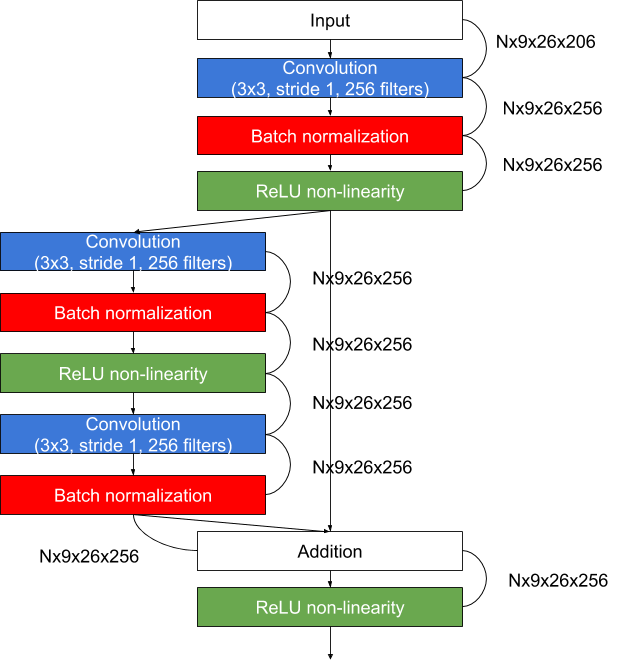
\includegraphics[scale=0.3]{../figures/architecture}
    \caption{Architecture Diagram for shared processing of the state space features. An initial convolution block is used to standardize the number of features, which is then followed by 18 residual blocks.}
    \label{fig:input_architecture_diagram}
\end{figure}

\begin{table}[h!]
\begin{tabular}{|l|l|l|}
\hline
\textit{\textbf{Domain}} & \textbf{Input Dimensions} & \textbf{Total Size} \\ \hline
\textbf{Atari 2600}      & 84 x 84 x 4               & 28,224              \\ \hline
\textbf{Go}              & 19 x 19 x 17              & 6,137               \\ \hline
\textbf{Chess}           & 8 x 8 x 119               & 7,616               \\ \hline
\textbf{Shogi}           & 9 x 9 x 362               & 29,322              \\ \hline
\textbf{Terra Mystica}   & 9 x 26 x 206              & 48,204              \\ \hline
\textbf{ImageNet}        & 224x224x1                 & 50,176              \\ \hline
\end{tabular}
\caption{Comparison of input sizes for different domain of both games. For reference, typical CNN domain of ImageNet is also included.}
\label{table:input_size_comparison}
\end{table}

\begin{table}[h!]
\begin{tabular}{|l|l|l|}
\hline
\textit{\textbf{Domain}} & \textbf{Input Dimensions} & \textbf{Total Size} \\ \hline
\textbf{Atari 2600}      & 18 x 1               & 18              \\ \hline
\textbf{Go}              & 19 x 19 + 1              & 362               \\ \hline
\textbf{Chess}           & 8 x 8 x 73               & 4,672               \\ \hline
\textbf{Shogi}           & 9 x 9 x 139               & 11,259              \\ \hline
\textbf{Terra Mystica}   & 9 x 13 x 18 + 4x3 + 25 &   2,143            \\ \hline
\textbf{ImageNet}        & 1000x1                 & 1000              \\ \hline
\end{tabular}
\caption{Comparison of action space sizes for different domain of both games. For ImageNet, we consider the class-distribution the actions-space}
\label{table:output_size_comparison}
\end{table}


\begin{table}[h!]
\begin{tabular}{|l|l|l|}
\hline
\multicolumn{3}{|c|}{{\ul \textbf{Average Human Score (2p)}}}      \\ \hline
\textbf{Faction} & \textbf{Average Score} & \textbf{Sampled Games} \\ \hline
Halfing          & 133.32                 & 2227                   \\ \hline
Engineers        & 127.72                 & 1543                   \\ \hline
\end{tabular}
\caption{Average human scores by faction for a two-player TM games online.}
\label{table:average_2p_score}
\end{table}

\begin{table}[h!]
\begin{tabular}{|l|l|l|}
\hline
\multicolumn{3}{|c|}{{\ul \textbf{Simulated Self-Play Average Scores}}}      \\ \hline
\textbf{Faction} & \textbf{Average Score} & \textbf{Sampled Games} \\ \hline
Halfing          & 92.21                 & 1000                   \\ \hline
Engineers        & 77.12                 & 1000                   \\ \hline
\end{tabular}
\caption{Self-play easy AI agent: AI\_Level5 from \cite{TMStatsAI}}
\label{table:average_2p_score}
\end{table}

\begin{table}[h!]
\begin{tabular}{|l|l|l|l|}
\hline
\multicolumn{3}{|c|}{{\ul \textbf{Simulated Self-Play Average Scores}}}      \\ \hline
\textbf{Faction} & \textbf{Average Score\footnote{Over Final 1000 Games of Self-Play}} & \textbf{Training Iterations} \\ \hline
Halfing          & 32.11                 & 10,000                   \\ \hline
Engineers        & 34.12                 & 10,000                 \\ \hline
\end{tabular}
\caption{Our Self-Play AI after 10,000 training iterations, with average score over final 1000 games.}
\label{table:average_2p_score_our_ai}
\end{table}


\begin{figure}[h!]
    \centering
    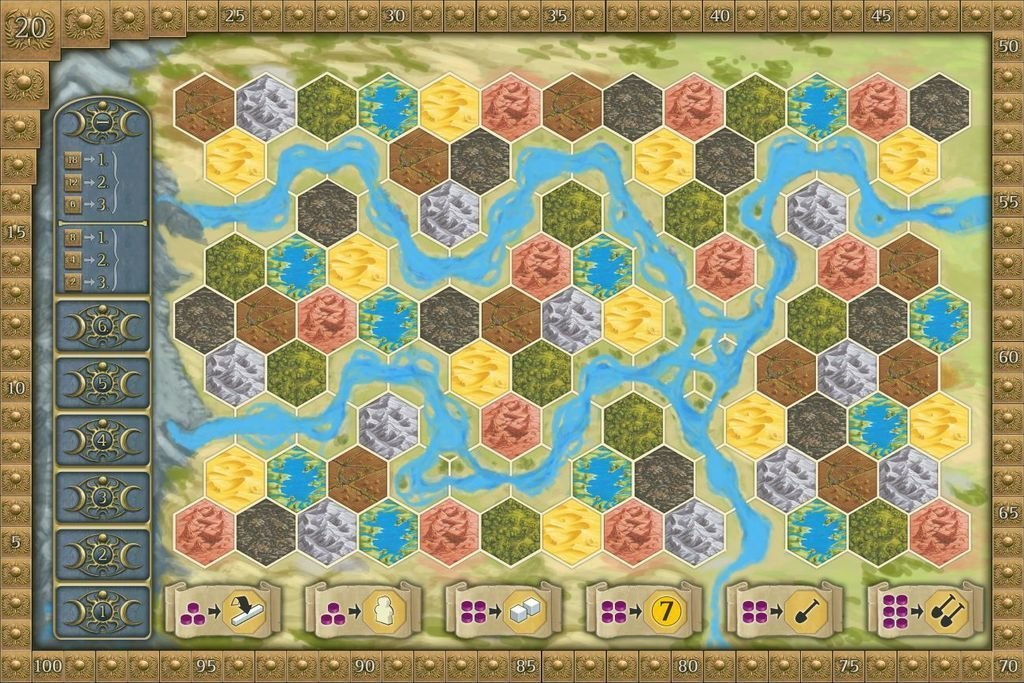
\includegraphics[scale=0.2]{../figures/tm_board}
    \caption{The Terra Mystica Game Board and Its Representation}
    \label{fig:TM_Board}
\end{figure}

\begin{figure}[h!]
    \centering
    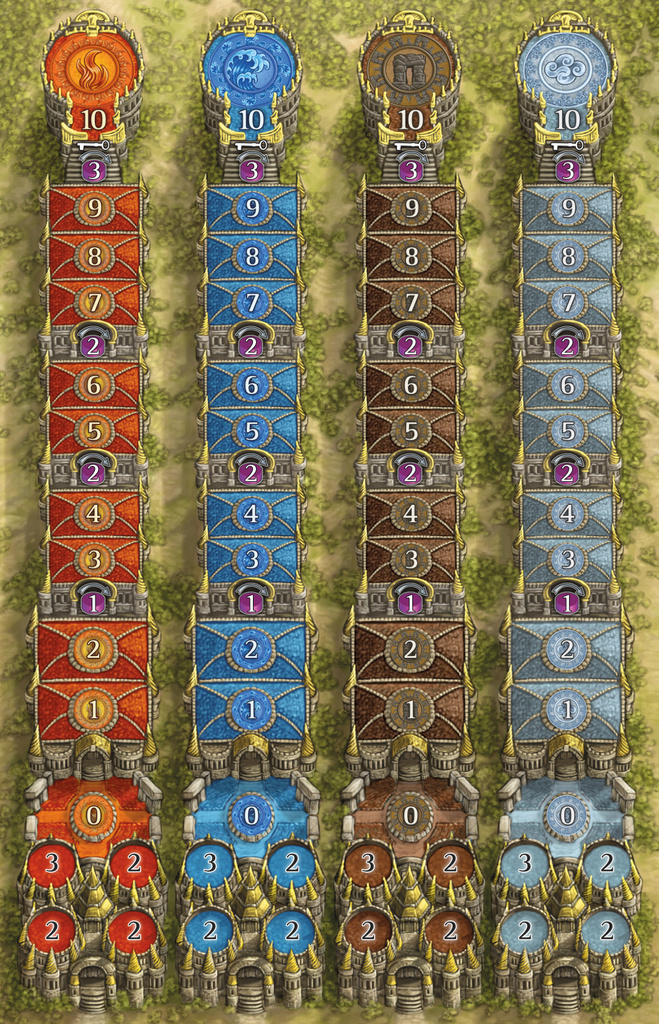
\includegraphics[scale=0.6]{../figures/terra-mystica-cult}
    \caption{The Terra Mystica Cult Track}
    \label{fig:TM_Cult_Track}
\end{figure}

\begin{figure}[h!]
    \centering
    \includegraphics[scale=0.6]{../figures/image_tm-cult}
    \caption{The Terra Mystica Cult Track}
    \label{fig:TM_Board_Representation}
\end{figure}

{\small
\bibliographystyle{../common/ieee}
\bibliography{../common/egbib}
}

\end{document}
